Auch ohne äußere elektrische Felder bewegen sich freie Ladungsträger im Gas aufgrund ihrer
thermischen Energie. Diese Bewegung entspricht einer Maxwell-Verteilung. Für Ionen gilt

\[\langle E_{\text{kin}} \rangle = \frac{1}{2} m \langle u^2 \rangle ~~~~~\text{mit}~~~~ \langle u^2
\rangle = \frac{3kT}{m}
\]

Ausgangspunkt ist eine punktförmige Ladungsverteilung, die in eine zerfließende Gaußverteilung
übergeht.

\begin{figure}[H]
	\centering
	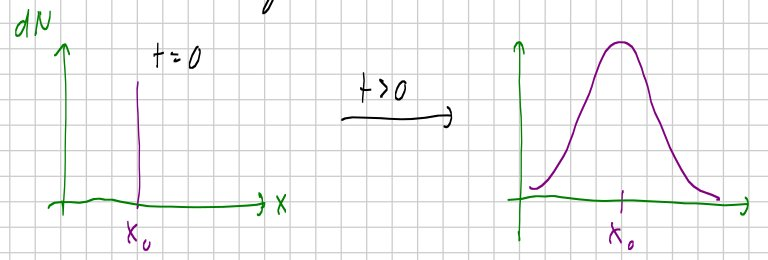
\includegraphics[width=0.5\textwidth]{gausskurve2.jpg}
\end{figure}

Dieser Prozess wird beschrieben durch

\[\frac{\mathrm{d}N}{N} = \frac{1}{\sqrt{4\pi\cdot D\cdot t}}\,
\text{exp}\left(-\frac{x^2}{4\,D\cdot t}\right)\,\mathrm{d}x
\]

wobei die Breite $\sigma_x=\sqrt{2D\cdot t}$ durch den Diffusionskoeffizienten $D$ beschrieben wird.
Je schneller die Teilchen sind, desto größer wird $D$. Insbesondere nimmt $\langle u^2 \rangle \sim
\frac{1}{m}$ mit abnehmender Teilchenmasse zu.
\\
Die mittlere freie Weglänge während des Diffusionsprozesses ist 

\[\lambda(E_{\text{kin}}) = \frac{1}{\frac{N_0\cdot\rho}{A}\cdot \sigma(E_{\text{kin}})} ,\]

also eine Funktion der kinetischen Energie des geladenen Teilchens.
\\
Die zuvor angegebene Breite der Gaußverteilung galt für die Diffusion in einer Dimension. In drei
Dimensionen gilt

\[\sigma = \sqrt{6D\cdot t} . \]

Der Diffusionskoeffizient kann in der kinetischen Gastheorie berechnet werden:

\[D=\frac{1}{3} \langle u \rangle \cdot \lambda~~~~~\text{mit}~~~~\langle u \rangle
=\sqrt{\frac{8\,k\cdot T}{\pi\cdot m}}\]

und $\lambda$ als mittlere freie Weglänge des Ladungsträgers. Damit ergibt sich das folgende Bild
für die expliziten Abhängigkeiten von $D$:

\[ D= \frac{2}{3\sqrt{\pi}}\cdot \frac{1}{\rho\cdot\sigma_0}\sqrt{\frac{(k\cdot T)^3}{m}} \]

\begin{itemize}
  \item $D\sim 1/\sqrt{m}$
  \item $D\sim \sqrt{T^3}$
  \item $D\sim 1/\rho$
\end{itemize}

Dabei ist $\sigma_0$ der totale Stoßwirkungsquerschnitt des Ladungsträgers mit einem Gasmolekül.
